\appendix
\chapter{Realisierung des Prototypen}

\begin{figure}[ht]
	\centering
	\subfigure[Prototyp - Übersicht aller Außenlichtoptionen]{\includegraphics[width=0.49\textwidth]{SS_Overview}}
	\subfigure[Prototyp - Detailansicht einer Außenlichtoption]{\includegraphics[width=0.49\textwidth]{SS_Detail}}
	\caption{Prototyp: Übersicht der Lichtoptionen und Detailansicht}
\end{figure}

\begin{figure}[ht]
	\centering
	\subfigure[Prototyp - Kauf einer Außenlichtoption mit Apple Pay]{\includegraphics[width=0.49\textwidth]{SS_ApplePay}}
	\subfigure[Prototyp - Übersicht aller Credits-Pakete]{\includegraphics[width=0.49\textwidth]{SS_Credits}}
	\caption{Prototyp: Kauf einer Lichtoption und eines Credits-Paktes}
\end{figure}

\begin{figure}[ht]
	\centering
	\subfigure[Prototyp - Auswahl der Währung beim Kauf]{\includegraphics[width=0.49\textwidth]{SS_Buy}}
	\subfigure[Prototyp - Auswahl der Währung beim Abonnieren]{\includegraphics[width=0.49\textwidth]{SS_Subscription}}
	\caption{Prototyp: Auswahl der Währung}
\end{figure}

\chapter{Klassendiagramme}
\label{appendix:KD}
\begin{figure}[ht]
	\centering
		\subfigure[Klassendiagramm: DatabaseController]{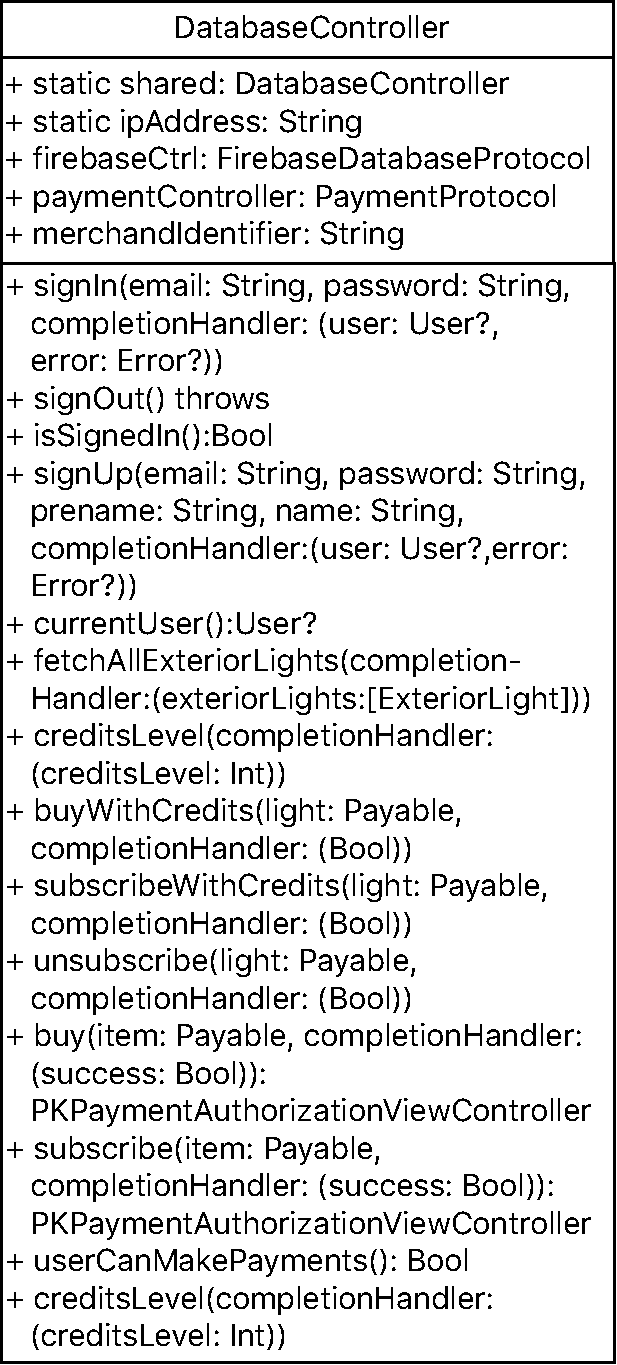
\includegraphics[width=0.45\textwidth]{KD_DatabaseController}}
	\subfigure[Klassendiagramm: ApplePayButton]{\includegraphics[width=0.45\textwidth]{KD_ApplePayButton}}
	\caption{Klassendiagramme: DatabaseProtocol und ApplePayButton}
	\label{appendix:KD:DatabaseCtrlApplePay}
\end{figure}


\begin{figure}[ht]
	\centering
	\subfigure[Klassendiagramm: CreditsPaymentProtocol]{\includegraphics[width=0.47\textwidth]{KD_CreditsPayment}}
		\subfigure[Klassendiagramm: CreditsPackage]{\includegraphics[width=0.49\textwidth]{KD_CreditsPackage}}
	\caption{Klassendiagramme: CreditsPaymentProtocol und CreditsPackage}
	\label{appendix:KD:CreditsPaymentCreditsPackage}
\end{figure}


\begin{figure}[ht]
	\centering
		\subfigure[Klassendiagramm: ExteriorLight]{\includegraphics[width=0.49\textwidth]{KD_ExteriorLight}}
		\subfigure[Klassendiagramm: PaymentController]{\includegraphics[width=0.49\textwidth]{KD_PaymentController}}
	\caption{Klassendiagramme: ExteriorLight und PaymentController}
	\label{appendix:KD:ExteriorLightPaymentController}
\end{figure}


\begin{figure}[ht]
	\centering
	\subfigure[Klassendiagramm: FirebaseDatabaseController]{\includegraphics[width=0.49\textwidth]{KD_FirebaseDatabaseController}}
	\subfigure[Klassendiagramm: LightProtocol]{\includegraphics[width=0.49\textwidth]{KD_LightProtocol}}
	\caption{Klassendiagramme: FirebaseDatabaseController und LightProtocol}
	\label{appendix:KD:FirebaseDatabaseCtrlLightProtocol}
\end{figure}

\begin{figure}[ht]
	\centering
	\subfigure[Klassendiagramm: MoneyPaymentProtocol]{\includegraphics[width=0.49\textwidth]{KD_MoneyPaymentProtocol}}
	\subfigure[Klassendiagramm: PKPaymentAuthorizationViewControllerDelegate]{\includegraphics[width=0.49\textwidth]{KD_PKPaymentAuthorizationViewControllerDelegate}}
	\caption{Klassendiagramme: MoneyPaymentProtocol und PKPaymentAuthorizationViewControllerDelegate}
	\label{appendix:KD:MoneyPaymentPKPayment}
\end{figure}

\begin{figure}[ht]
	\centering
		\subfigure[Klassendiagramm: PaymentProtocol]{\includegraphics[width=0.49\textwidth]{KD_PaymentProtocol}}
	\subfigure[Klassendiagramm: DecodeableProtocol]{\includegraphics[width=0.49\textwidth]{KD_DecodeableProtocol}}
	\caption{Klassendiagramme: PaymentProtocol und DecodeableProtocol}
	\label{appendix:KD:PaymentProtocolDecodeableProtocol}
\end{figure}

\begin{figure}[ht]
	\centering
			\subfigure[Klassendiagramm: User]{\includegraphics[width=0.47\textwidth]{KD_User}}
\subfigure[Klassendiagramm: PackageProtocol]{\includegraphics[width=0.47\textwidth]{KD_PackageProtocol}}
	\caption{Klassendiagramme: User und PackageProtocol}
	\label{appendix:KD:UserPackageProtocol}
\end{figure}



